\chapter{列表}

\index{列表}
\index{类型!列表}


\section{列表是一个序列}

类似字符串,{\bf 列表}一个序列的值。在字符串中,每个值是字符;在一个列表中可以是任何数据类型。列表中的数值称为{\bf 元素},有时也称为{\bf 项目}。

\index{元素}
\index{序列}
\index{项目}

有多种方法可以创建一个新的列表;最简单的方法是用方括号(\verb"["和\verb"]")将元素包括起来:

\beforeverb
\begin{verbatim}
[10, 20, 30, 40]
['crunchy frog', 'ram bladder', 'lark vomit']
\end{verbatim}
\afterverb
%
第一个例子是包含4个整数的列表。第二个例子是包含3个字符串的列表。一个列表中的元素不需要是相同数据类型。下面的列表包含一个字符串、一个浮点数、一个整数和另一个列表:

\beforeverb
\begin{verbatim}
['spam', 2.0, 5, [10, 20]]
\end{verbatim}
\afterverb
%
在一个列表中的列表称为{\bf 嵌套}。

\index{嵌套列表}
\index{列表!嵌套}

没有任何元素的列表称为空列表。你可以使用空的括号\verb"[]"创建一个空列表。

\index{空列表}
\index{列表!空}

正如你可能期望的,列表的值可以被赋值给变量:

\beforeverb
\begin{verbatim}
>>> cheeses = ['Cheddar', 'Edam', 'Gouda']
>>> numbers = [17, 123]
>>> empty = []
>>> print cheeses, numbers, empty
['Cheddar', 'Edam', 'Gouda'] [17, 123] []
\end{verbatim}
\afterverb
%

\index{赋值}

% From Jeff: write sum for a nested list?


\section{列表是可改变的}

\index{列表!元素}
\index{访问}
\index{下标}
\index{括号运算符}
\index{运算符!括号}

访问列表中元素的语法和访问字符串中字符的语法相同,都是通过括号运算符实现的。括号中的表达式指定了下标。记住下标从0开始:

\beforeverb
\begin{verbatim}
>>> print cheeses[0]
Cheddar
\end{verbatim}
\afterverb
%
与字符串不同,列表是可以改变的。当括号运算符出现在赋值语句的左边,它指向列表中将被赋值的元素。

\index{可改变的}

\beforeverb
\begin{verbatim}
>>> numbers = [17, 123]
>>> numbers[1] = 5
>>> print numbers
[17, 5]
\end{verbatim}
\afterverb
%
{\tt numbers}中的第一个元素,原来是123,现在是5。
used to be 123, is now 5.

\index{下标!从0开始}
\index{0,下标开始于}

你可以将列表看成下标和元素的对应关系。这种关系成为{\bf 映射}。每个下标“对应”一个元素。这里给出{\tt cheeses},{\tt numbers}和{\tt empty}的状态图:

\index{状态图}
\index{图!状态}
\index{映射}

\beforefig
\centerline{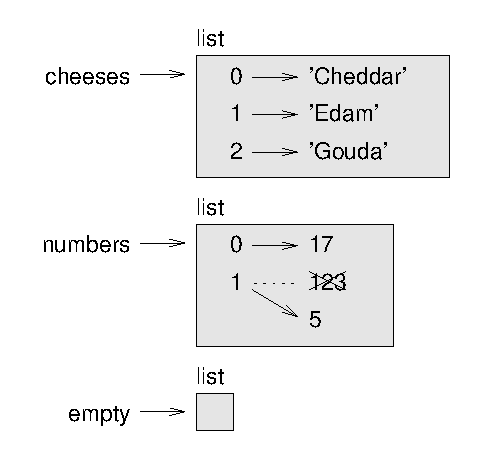
\includegraphics{figs/list_state.eps}}
\afterfig

列表用外部标有“list”的盒子表示,内部是列表中的元素。{\tt cheeses}是一个有3个元素的列表,下标分别是0,1和2。{\tt numbers}包含2个元素。状态图显示了第二个元素原来是123,被重新赋值为5。{\tt empty}对应一个没有元素的列表。

\index{项目赋值}
\index{赋值!项目}

列表下标的工作原理和字符串的相同:

\begin{itemize}

\item 任何整数表达式可以作为下标。

\item 试图读写一个不存在的元素将得到{\tt 下标错误}。

\index{异常!下标错误}
\index{下标错误}

\item 下标可以取负数,它将从后往前访问列表。

\end{itemize}

\index{列表!下标}


\index{列表!成员}
\index{成员!列表}
\index{in运算符}
\index{运算符!in}

{\tt in}运算符同样使用列表。

\beforeverb
\begin{verbatim}
>>> cheeses = ['Cheddar', 'Edam', 'Gouda']
>>> 'Edam' in cheeses
True
>>> 'Brie' in cheeses
False
\end{verbatim}
\afterverb


\section{遍历列表}
\index{列表!遍历}
\index{遍历!列表}
\index{for循环}
\index{循环!for}
\index{语句!for}

最常用的遍历列表的方式是使用{\tt for}循环。语法类似字符串:

\beforeverb
\begin{verbatim}
for cheese in cheeses:
    print cheese
\end{verbatim}
\afterverb
%
这种写法适用于只读列表中的元素。如果你需要写或者更新元素,你需要通过下标访问。一个常用的做法是结合{\tt range}和{\tt len}函数:

\index{循环!下标}
\index{下标!循环}

\beforeverb
\begin{verbatim}
for i in range(len(numbers)):
    numbers[i] = numbers[i] * 2
\end{verbatim}
\afterverb
%
这个循环遍历列表并更新每个元素。{\tt len}函数返回列表中元素个数。{\tt range}函数返回一个从0到$n-1$的下标的列表,其中$n$是列表的长度。每次循环中,{\tt i}得到下一个元素的下标。循环主体中的赋值语句使用{\tt i}读取老的值并赋值新的值。

\index{项目更新}
\index{更新!项目}

对于一个空列表的{\tt for}循环将不会执行循环的主体:

\beforeverb
\begin{verbatim}
for x in empty:
    print 'This never happens.'
\end{verbatim}
\afterverb
%
虽然一个列表可以包含另一个列表,被嵌套的列表作为单独的一个元素。以下列表的长度为4:

\index{嵌套列表}
\index{列表!嵌套}

\beforeverb
\begin{verbatim}
['spam', 1, ['Brie', 'Roquefort', 'Pol le Veq'], [1, 2, 3]]
\end{verbatim}
\afterverb



\section{列表操作}
\index{列表!操作}

运算符{\tt +}连接列表:

\index{连接!列表}
\index{列表!连接}

\beforeverb
\begin{verbatim}
>>> a = [1, 2, 3]
>>> b = [4, 5, 6]
>>> c = a + b
>>> print c
[1, 2, 3, 4, 5, 6]
\end{verbatim}
\afterverb
%
类似的,运算符{\tt *}给定次数地重复列表:

\index{重复!列表}
\index{列表!重复}

\beforeverb
\begin{verbatim}
>>> [0] * 4
[0, 0, 0, 0]
>>> [1, 2, 3] * 3
[1, 2, 3, 1, 2, 3, 1, 2, 3]
\end{verbatim}
\afterverb
%
第一个例子重复{\tt [0]}4次。第二个例子重复列表{\tt [1, 2, 3]}3次。


\section{列表切片}

\index{切片运算符}
\index{运算符!切片}
\index{下标!切片}
\index{列表!切片}
\index{切片!列表}

切片运算符同样适用于列表:

\beforeverb
\begin{verbatim}
>>> t = ['a', 'b', 'c', 'd', 'e', 'f']
>>> t[1:3]
['b', 'c']
>>> t[:4]
['a', 'b', 'c', 'd']
>>> t[3:]
['d', 'e', 'f']
\end{verbatim}
\afterverb
%
如果你忽略第一个下标,切片从列表头开始。如果你忽略第二个,切片到列表尾部结束。因此如果你忽略两个,切片为整个列表的拷贝。

\index{列表!复制}
\index{切片!复制}
\index{复制!切片}

\beforeverb
\begin{verbatim}
>>> t[:]
['a', 'b', 'c', 'd', 'e', 'f']
\end{verbatim}
\afterverb
%
由于列表是可改变的,有必要在折叠、旋转或切断操作前复制列表。

\index{可改变}

赋值语句左边的切片运算符可以更新多个元素:

\index{slice!update}
\index{update!slice}

\beforeverb
\begin{verbatim}
>>> t = ['a', 'b', 'c', 'd', 'e', 'f']
>>> t[1:3] = ['x', 'y']
>>> print t
['a', 'x', 'y', 'd', 'e', 'f']
\end{verbatim}
\afterverb
%

% You can add elements to a list by squeezing them into an empty
% slice:

% \beforeverb
% \begin{verbatim}
% >>> t = ['a', 'd', 'e', 'f']
% >>> t[1:1] = ['b', 'c']
% >>> print t
% ['a', 'b', 'c', 'd', 'e', 'f']
% \end{verbatim}
% \afterverb
%
% And you can remove elements from a list by assigning the empty list to
% them:

% \beforeverb
% \begin{verbatim}
% >>> t = ['a', 'b', 'c', 'd', 'e', 'f']
% >>> t[1:3] = []
% >>> print t
% ['a', 'd', 'e', 'f']
% \end{verbatim}
% \afterverb
%
% But both of those operations can be expressed more clearly
% with list methods.


\section{列表方法}

\index{列表!方法}
\index{方法,列表}

Python提供了一个列表的方法。例如,{\tt append}方法将新的元素添加到列表尾部:

\index{append方法}
\index{方法!append}

\beforeverb
\begin{verbatim}
>>> t = ['a', 'b', 'c']
>>> t.append('d')
>>> print t
['a', 'b', 'c', 'd']
\end{verbatim}
\afterverb
%
{\tt extend}方法读取一个列表作为参数,并附加其中所有的元素:

\index{extend方法}
\index{方法!extend}

\beforeverb
\begin{verbatim}
>>> t1 = ['a', 'b', 'c']
>>> t2 = ['d', 'e']
>>> t1.extend(t2)
>>> print t1
['a', 'b', 'c', 'd', 'e']
\end{verbatim}
\afterverb
%
这个例子中{\tt t2}没有改变。

{\tt sort}方法从小到大对列表中的元素进行排序:

\index{sort方法}
\index{方法!sort}

\beforeverb
\begin{verbatim}
>>> t = ['d', 'c', 'e', 'b', 'a']
>>> t.sort()
>>> print t
['a', 'b', 'c', 'd', 'e']
\end{verbatim}
\afterverb
%
列表的方法都是空的,它们对列表进行修改并返回{\tt None}。如果你写了{\tt t = t.sort()},你不会得到你想要的结果。

\index{空方法}
\index{方法!空}
\index{特殊值None}
\index{特殊值!None}


\section{映射,筛选和归并}

对列表中所有元素求和,你可以这么使用循环:

% see add.py

\beforeverb
\begin{verbatim}
def add_all(t):
    total = 0
    for x in t:
        total += x
    return total
\end{verbatim}
\afterverb
%
{\tt total}被初始化为0。每次经过循环,{\tt x}从列表中读取一个元素。运算符{\tt +=}提供可一个快捷的更新变量的方法。这是{\bf 增量赋值语句}:

\index{更新运算符}
\index{运算符!更新}

\index{赋值!增量}
\index{增量赋值}

\beforeverb
\begin{verbatim}
    total += x
\end{verbatim}
\afterverb
%
相当于:

\beforeverb
\begin{verbatim}
    total = total + x
\end{verbatim}
\afterverb
%
当循环执行时,{\tt total}记录了元素的和。这样的变量称为{\bf 累加器}。

\index{累加器!和}

对列表中元素求和是一个普通的操作,Python提供了内建函数{\tt sum}:

\beforeverb
\begin{verbatim}
>>> t = [1, 2, 3]
>>> sum(t)
6
\end{verbatim}
\afterverb
%
类似将一个序列的元素合并到一个单一的数值的操作称为{\bf 归并}。

\index{归并模式}
\index{模式!归并}
\index{遍历}


有时你需要遍历一个列表来构建另一个列表。例如,下面的函数读取一个字符串列表作为参数,返回大写后的新列表:

\beforeverb
\begin{verbatim}
def capitalize_all(t):
    res = []
    for s in t:
        res.append(s.capitalize())
    return res
\end{verbatim}
\afterverb
%
{\tt res}被初始化为一个空的列表。每次循环中,我们附加下一个元素。因此{\tt res}是另一种累加器。

\index{累加器!列表}
类似\verb"capitalize_all"有时被称为{\bf 映射},因为它对序列中的每个元素“映射”某个函数(在本例中是方法{\tt capitalize})。

\index{映射模式}
\index{模式!映射}
\index{筛选模式}
\index{模式!筛选}

另一个常见的操作是从列表中选择一些元素,并返回一个子列表。例如,下面的函数读取一个字符串列表,并返回仅包含大写字符串的列表:

\beforeverb
\begin{verbatim}
def only_upper(t):
    res = []
    for s in t:
        if s.isupper():
            res.append(s)
    return res
\end{verbatim}
\afterverb
%
{\tt isupper}是一个字符串的方法,如果字符串仅含有大写字母,则返回{\tt True}。

类似\verb"only_upper"的操作被称为{\bf 筛选},它选出一部分元素,而过滤其他元素。

绝大多数列表操作可以表示为映射、筛选和归并的组合。由于这些操作很常用,Python提供了语言特点的支持,包括内建函数{\tt map}和一个称为“列表理解”的运算符。

\index{列表!理解}

\begin{ex}
\label{累积}
\index{累积求和}

编写函数,读取一个数字列表作为参数,返回累积求和值。即第$i$个元素是原列表中前$i+1$个元素的和。例如,{\tt [1, 2, 3]}的累积求和为{\tt [1, 3, 6]}。
\end{ex}


\section{删除元素}

\index{元素删除}
\index{删除,列表中的元素}

有多种方法从列表中删除一个元素。如果你知道元素的下标,你可以使用{\tt pop}:

\index{pop方法}
\index{方法!pop}

\beforeverb
\begin{verbatim}
>>> t = ['a', 'b', 'c']
>>> x = t.pop(1)
>>> print t
['a', 'c']
>>> print x
b
\end{verbatim}
\afterverb
%
{\tt pop}修改列表,并返回被删除的元素。如果你不提供下标,它将删除最后一个元素。

如果你不需要被删除的值,你可以使用{\tt del}运算符:

\index{del运算符}
\index{运算符!del}

\beforeverb
\begin{verbatim}
>>> t = ['a', 'b', 'c']
>>> del t[1]
>>> print t
['a', 'c']
\end{verbatim}
\afterverb
%
如果你知道你要删除的元素(但不知道下标),你可以使用{\tt remove}:

\index{remove方法}
\index{方法!remove}

\beforeverb
\begin{verbatim}
>>> t = ['a', 'b', 'c']
>>> t.remove('b')
>>> print t
['a', 'c']
\end{verbatim}
\afterverb
%
{\tt remove}的返回值是{\tt None}。

\index{特殊值None}
\index{特殊值!None}

要删除多于一个元素,你可以对{\tt del}使用切片下标:

\beforeverb
\begin{verbatim}
>>> t = ['a', 'b', 'c', 'd', 'e', 'f']
>>> del t[1:5]
>>> print t
['a', 'f']
\end{verbatim}
\afterverb
%
照常,切片选择从第一个下标到第二个下标(不包括第二个下标)中的所有元素。


\section{列表和字符串}

\index{列表}
\index{字符串}
\index{序列}

字符串是字符的序列,列表是值的序列,但是字符的列表不同于字符串。你可以使用{\tt list}将字符串转化为字符的列表:

\index{list!函数}
\index{函数!list}

\beforeverb
\begin{verbatim}
>>> s = 'spam'
>>> t = list(s)
>>> print t
['s', 'p', 'a', 'm']
\end{verbatim}
\afterverb
%
由于{\tt list}是内建函数名,你应该避免将它作为变量名。我同样避免使用{\tt l}因为它看起来像{\tt 1}。于是我用了{\tt t}。

{\tt list}函数将字符串分割成单独的字符。如果你要将字符串分割成单词,你可以使用{\tt split}方法:

\index{split方法}
\index{方法!split}

\beforeverb
\begin{verbatim}
>>> s = 'pining for the fjords'
>>> t = s.split()
>>> print t
['pining', 'for', 'the', 'fjords']
\end{verbatim}
\afterverb
%
一个可选的参数称为{\bf 分割符},它指定了什么字符作为分界线。下面的例子使用连字符作为分割符:

\index{可选参数}
\index{参数!可选}
\index{分割服}

\beforeverb
\begin{verbatim}
>>> s = 'spam-spam-spam'
>>> delimiter = '-'
>>> s.split(delimiter)
['spam', 'spam', 'spam']
\end{verbatim}
\afterverb
%
{\tt join}功能和{\tt split}相反。它将一个列表字符串连接起来。{\tt join}是一个字符串方法,因此你需要在一个分割符上调用它,并传递一个列表作为参数:

\index{join方法}
\index{方法!join}
\index{连接}

\beforeverb
\begin{verbatim}
>>> t = ['pining', 'for', 'the', 'fjords']
>>> delimiter = ' '
>>> delimiter.join(t)
'pining for the fjords'
\end{verbatim}
\afterverb
%
在这个例子中分割符是一个空格,{\tt join}在每个单词中间添加一个空格。如果不需要使用空格连接,你可以使用一个空的字符串\verb"''"作为分割符。

\index{空字符串}
\index{字符串!空}


\section{对象和值}

\index{对象}
\index{值}

如果我们执行以下的赋值语句:

\beforeverb
\begin{verbatim}
a = 'banana'
b = 'banana'
\end{verbatim}
\afterverb
%
我们知道{\tt a}和{\tt b}都指向一个字符串,但我们不知道他们是否指向一个{\em 相同的}字符串。有些两种可能:

\index{别名}

\beforefig
\centerline{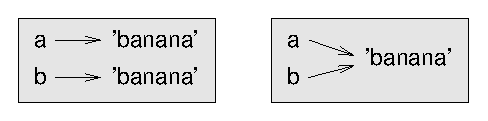
\includegraphics{figs/list1.eps}}
\afterfig

在第一种情况中,{\tt a}和{\tt b}指向两个有相同值的不同对象。在第二种情况中,它们指向同一个对象。

\index{is运算符}
\index{运算符!is}

你可以使用{\tt is}运算符检查两个变量是否指向同一个对象:

\beforeverb
\begin{verbatim}
>>> a = 'banana'
>>> b = 'banana'
>>> a is b
True
\end{verbatim}
\afterverb
%
在这个例子中,Python只产生了一个字符串对象,{\tt a}和{\tt b}都指向它。

但是如果你创建两个列表,你得到两个对象:

\beforeverb
\begin{verbatim}
>>> a = [1, 2, 3]
>>> b = [1, 2, 3]
>>> a is b
False
\end{verbatim}
\afterverb
%
状态图看起来是这样的:

\index{状态图}
\index{图!状态}

\beforefig
\centerline{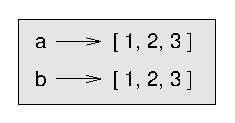
\includegraphics{figs/list2.eps}}
\afterfig

在本例中,我们称这两个列表是{\bf 相等的},因为它们有相同的元素,但不是{\bf 相同的},因为它们不是同一个对象。如果两个对象是相同的,它们也是相等的,但是如果它们是相等的,它们不一定相同。

\index{相等}
\index{相同}

目前为止,我们可以交换地使用“对象”和“值”,但更精确地说是对象包含一个值。如果你执行{\tt [1,2,3]},你会得到一个整数序列的对象。如果另一个列表有相同的元素,我们称它有相同的值,但它不是相同的对象。

\index{对象}
\index{值}


\section{别名}

\index{别名}
\index{引用!别名}

如果{\tt a}指向一个对象,然后你进行赋值{\tt b = a},那么两个变量都指向同一个对象:

\beforeverb
\begin{verbatim}
>>> a = [1, 2, 3]
>>> b = a
>>> b is a
True
\end{verbatim}
\afterverb
%
状态图如图所示:

\index{状态图}
\index{图!状态}

\beforefig
\centerline{
\includegraphics{figs/list3.eps}}
\afterfig

一个变量和一个对象的关联称为{\bf 引用}。在这个例子中,同一个对象有两个引用。

\index{引用}

如果一个对象有多于一个引用,我们称这个对象是有{\bf 别名}的。

\index{可改变}
有别名的对象是可改变的,对一个别名的改动会影响另一个:

\beforeverb
\begin{verbatim}
>>> b[0] = 17
>>> print a
[17, 2, 3]
\end{verbatim}
\afterverb
%
这个行为虽然很有用,但容易造成错误。通常,对于可改变的对象避免使用别名相对更安全。

\index{不可改变}

对于不可改变的对象,如字符串,使用别名没有任何问题。例如:

\beforeverb
\begin{verbatim}
a = 'banana'
b = 'banana'
\end{verbatim}
\afterverb
%
使用{\tt a}或者{\tt b}指向同一个字符串基本上没有任何区别。


\section{列表参数}

\index{列表!作为参数}
\index{参数}
\index{参数!列表}
\index{引用}
\index{参数}

当你将一个列表作为参数传给一个函数,函数将得到这个列表的一个引用。如果函数对这个列表参数进行了修改,调用者会看见变动。例如,\verb"delete_head"删除列表的第一个元素:

\beforeverb
\begin{verbatim}
def delete_head(t):
    del t[0]
\end{verbatim}
\afterverb
%
它是这么使用的:

\beforeverb
\begin{verbatim}
>>> letters = ['a', 'b', 'c']
>>> delete_head(letters)
>>> print letters
['b', 'c']
\end{verbatim}
\afterverb
%
参数{\tt t}和变量{\tt letters}是同一个对象的别名。栈图如下:

\index{栈图}
\index{图!栈}

\beforefig
\centerline{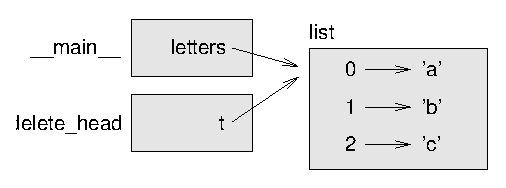
\includegraphics{figs/stack5.eps}}
\afterfig

由于列表被两个帧共享,我把它画在它们中间。

需要注意的是修改列表操作和创建列表操作间的区别,例如,{\tt append}方法是修改一个列表,而{\tt +}运算符是创建一个新的列表:

\index{append方法}
\index{方法!append}
\index{列表!连接}
\index{连接!列表}

\beforeverb
\begin{verbatim}
>>> t1 = [1, 2]
>>> t2 = t1.append(3)
>>> print t1
[1, 2, 3]
>>> print t2
None

>>> t3 = t1 + [3]
>>> print t3
[1, 2, 3]
>>> t2 is t3
False
\end{verbatim}
\afterverb

如果你要编写函数修改列表,这个区别就很重要。例如,下面函数{\em 没有}删除列表的第一个元素:

\beforeverb
\begin{verbatim}
def bad_delete_head(t):
    t = t[1:]              # WRONG!
\end{verbatim}
\afterverb
切片操作创建一个新的列表,并使{\tt t}指向它。但这些操作对作为参数的列表都没有影响。

\index{切片运算符}
\index{运算符!切片}

一个替代的写法是创建并返回一个新的列表。例如,{\tt tail}返回不包含第一个元素的列表:

\beforeverb
\begin{verbatim}
def tail(t):
    return t[1:]
\end{verbatim}
\afterverb
%
这个函数并不修改原来的列表。下面给出如何使用这个函数:

\beforeverb
\begin{verbatim}
>>> letters = ['a', 'b', 'c']
>>> rest = tail(letters)
>>> print rest
['b', 'c']
\end{verbatim}
\afterverb


\begin{ex}

编写函数{\tt chop},读取一个列表并进行修改,删除第一个和最后一个元素,并返回{\tt None}。

再编写函数{\tt middle},读取一个列表作为参数,返回一个包含除了第一个和最后一个元素的新列表。

\end{ex}


\section{调试}
\index{调试}

粗心的使用列表(以及其他可改变的对象)会导致长时间的调试。下面给出一些常见的陷阱以及避免它们的方法:

\begin{enumerate}

\item 记住大多数的列表的方法对参数进行修改,然后返回{\tt None}。字符串的方法则相反,它们保留原始的字符串并返回一个新的字符串。

如果你习惯编写处理字符串的代码,如:

\beforeverb
\begin{verbatim}
word = word.strip()
\end{verbatim}
\afterverb

你可能会写出下面的代码:

\beforeverb
\begin{verbatim}
t = t.sort()           # WRONG!
\end{verbatim}
\afterverb

\index{sort方法}
\index{方法!sort}

由于{\tt sort}返回{\tt None},你对{\tt t}的下一个操作可能会失败。

在使用列表的方法和运算符前,你应该仔细阅读文档,并在交互模式下测试。列表和其他序列(如字符串)共有的方法和运算符的文档在\url{docs.python.org/lib/typesseq.html}。可改变的序列独有的方法和运算符的文档在\url{docs.python.org/lib/typesseq-mutable.html}。


\item 养成自己的编码习惯。

列表中的一个问题是有太多的途径做相同的事。例如,要删除列表中的一个元素,你可以使用{\tt pop},{\tt remove},{\tt del}甚至切片赋值。

要添加一个元素,你可以使用{\tt append}方法或{\tt +}运算符。但记住什么是正确的:

\beforeverb
\begin{verbatim}
t.append(x)
t = t + [x]
\end{verbatim}
\afterverb

以下是错误的:

\beforeverb
\begin{verbatim}
t.append([x])          # WRONG!
t = t.append(x)        # WRONG!
t + [x]                # WRONG!
t = t + x              # WRONG!
\end{verbatim}
\afterverb

在交互模式下测试每一个例子,保证你明白它们做了什么。注意只有最后一个会导致运行时错误,其他的都是合法的,但做了错误的事情。


\item 复制拷贝,避免别名。

\index{别名!复制以避免}
\index{赋值!以避免别名}

如果你要使用类似{\tt sort}的方法来修改参数,但同时有要保留原列表,你可以复制一个拷贝。

\beforeverb
\begin{verbatim}
orig = t[:]
t.sort()
\end{verbatim}
\afterverb

在这个例子中你还可以使用内建函数{\tt sorted},它将返回一个新的已排序的列表,原列表将保持不变。注意你需要避免使用{\tt sorted}作为变量名!

\end{enumerate}



\section{术语}

\begin{description}

\item[列表:] 一个序列的值。
\index{列表}

\item[元素:] 列表(或序列)中的一个值,也称为项目。
\index{元素}

\item[下标:] 对应列表中的元素的整数。
\index{下标}

\item[嵌套列表:] 列表中的元素是另一个列表。
\index{嵌套列表}

\item[列表遍历:] 对列表中的元素按顺序访问。
\index{列表!遍历}

\item[映射:] 一个集合中的元素和另一个集合中的元素的对应关系。例如,列表是下标到元素的映射。
\index{映射}

\item[累加器:] 循环中用于相加或累积的变量。
\index{累加器}

\item[增量赋值:] 更新变量的语句,使用类似\verb"+="的运算符。
\index{赋值!增量}
\index{增量赋值}

\index{遍历}

\item[归并:] 遍历序列,将所有元素求和为一个值的处理模式。
\index{归并模式}
\index{模式!归并}

\item[映射:] 遍历序列,对每个元素执行操作的处理模式。
\index{映射模式}
\index{模式!映射}

\item[筛选:] 遍历序列,选出满足一定标准的处理模式。
\index{筛选模式i}
\index{模式!筛选}

\item[对象:] 变量可以指向的东西。一个对象有其数据类型和值。
\index{对象}

\item[相等:] 有相同的值。
\index{相等}

\item[相同:] 是用一个对象(隐含相等)。
\index{相同}

\item[引用:] 变量和值间的关联。
\index{引用}

\item[别名:] 两个或两个以上的变量指向同一个对象。
\index{别名}

\item[分割符:] 用于指示字符串分割位置的字符或者字符串。
\index{分割符}

\end{description}


\section{练习}

\begin{ex}
编写函数\verb"is_sorted",读取一个列表作为参数,如果列表是升序排序的,则返回{\tt True},否则返回{\tt False}。你可以假设(作为先决条件)列表中的元素可以用关系运算符如{\tt <},{\tt >}等比较。

\index{先决条件}

例如,\verb"is_sorted([1,2,2])"将返回{\tt True},\verb"is_sorted(['b','a'])"将返回{\tt False}。
\end{ex}


\begin{ex}
\label{回文}

\index{回文}

两个单词是回文的,如果你可以重新排列一个的字符后可以拼写出另一个。编写函数\verb"is_anagram",读取两个字符串,如果它们是回文的则返回{\tt True}。
\end{ex}


\begin{ex}
\label{复制}

这也被称为生日悖论:

\begin{enumerate}

\index{生日悖论}
\index{赋值}

\item 编写函数\verb"has_duplicates",读取一个列表作为参数,如果任何元素出现超过一次,则返回{\tt True}。函数不能改变原列表。

\item 如果你班级上有23个学生,2个学生生日相同的概率是多少?你可以通过随即产生23个生日并检查匹配来估计概率。提示:你可以使用{\tt random}模块中的{\tt randint}函数来生成随即生日。

\index{random模块}
\index{模块!random}
\index{randint函数}
\index{函数!randint}

\end{enumerate}

你可以在\url{wikipedia.org/wiki/Birthday_paradox}了解这个问题,你可以在\url{thinkpython.com/code/birthday.py}找到我的程序。

\end{ex}


\begin{ex}

\index{赋值}
\index{唯一}

编写函数\verb"remove_duplicates",参数为一个列表,返回一个新的列表,其中只包含原列表中唯一的元素。提示:列表中的元素不一定按照原来的顺序。
\end{ex}


\begin{ex}
\index{append方法}
\index{方法append}
\index{列表!连接}
\index{连接!列表}

编写函数,读取文件{\tt words.txt},建立一个列表,每个单词为一个元素。编写两个版本函数,一个使用{\tt append}方法,另一个使用{\tt t = t + [x]}。那个版本运行得慢?为什么?

你可以在\url{thinkpython.com/code/wordlist.py}中找到我的程序。
\end{ex}


\begin{ex}
\label{单词表1}
\label{两分法}

\index{成员!两分法搜索}
\index{两分法搜索}
\index{搜索,两分法}

\index{成员!二进制搜索}
\index{二进制搜索}
\index{搜索,二进制}

检查一个单词是否在单词表中,你可以使用{\tt in}运算符,但这很慢,因为它按顺序查找单词。

由于单词是按照字母顺序排序的,我们可以使用两分法(也称二进制搜索)来加快速度,类似你在字典中查找单词的方法。你从中间开始,如果你要找的单词在中间的单词之前,你查找前半部分,否则你查找后半部分。

每次查找,你将搜索范围减小一半。如果单词表有113,809个单词,你只需要17步来找到这个单词,或着知道单词不存在。

编写函数{\tt bisect},参数为一个已排序的列表和一个目标值,返回该值在列表中的位置,如果不存在则返回{\tt None}。

\index{bisect模块}
\index{模块!bisect}

或者你可以阅读{\tt bisect}模块的文档并使用!
\end{ex}

\begin{ex}
\index{反转词对}

两个单词被称为是“反转词对”,如果一个是另一个的反转。编写函数,找出单词表中所有的反转词对。
\end{ex}

\begin{ex}
\index{连锁词}

两个单词被称为是“连锁词”,如果交替的从两个单词中取出字符将组成一个新的单词\footnote{这个练习来自\url{puzzlers.org}中的一个例子。}。例如,“shoe”和“cold”连锁后成为“schooled”。

\begin{enumerate}

\item 编写程序,找出所有的连锁词。提示:不用列举所有的单词对。

\item 你能够找到三重连锁的单词吗?即每个字母依次从3个单词得到。

\end{enumerate}
\end{ex}
